% !BIB TS-program = biber
% !BIB program = biber
% !TEX encoding = UTF-8
% !TEX program = lualatex
\documentclass[10pt,a4paper,twoside]{article}
\usepackage{../../../latex_packages/patomaki_style_twocolumn}
\changefontsizes[10pt]{10pt}
\renewcommand*{\bibfont}{\footnotesize}
\addbibresource{varactor_references.bib}
\title{\vspace{-2.5em}Impedance matching with cryogenic varactors in quantum dot reflectometry \vspace{-2em}} 
\date{}
\begin{document}
\maketitle
\begin{flushleft}
\textit{V. Ciriano, J. Duan, L. Keary, A. Owens, S. Patom{\"a}ki}
\\
\textit{University College London, Department of physics and astronomy}
\\
\textit{June 2018}
\end{flushleft}
\begin{multicols}{2}
% % 
% % 
\section{Introduction}
Carbon nanotubes (CNT) offer a promising platform for long lived quantum dots (QDs) compared to more traditional III-V semiconductor QDs, such as those made in GaAs. Coherence times in GaAs are limited by the fluctuating magnetic field environment created by the surrounding nuclear magnetic moments. Carbon and for example silicon atoms have zero nuclear magnetic moments, apart from naturally occuring impurities, such as $^{13}$C. In these materials, decoherence can be suppressed maximally by so-called isotopic purification. Lifetimes of ms have been measured in CNTs~\cite{CNTtime}, and dephasing times  of $\mu$s have been predicted. These are improvements by several orders of magnitude from the coherence times of tens of ns in e.g. GaAs QD qubits. However, CNT QD qubits are relatively underdeveloped, lacking essential features, such as single-shot readout. 
\par
%\begin{figure}[h]
%    \centering
%    \includegraphics[width=0.5\textwidth]{matching.png}
%    \caption{Matching circuit consisting of two variable varactors included as part of the quantum dot readout line.}
%    \label{fig:matching}
%\end{figure}
In this work we studied how the impedance matching in radio-frequency (RF) reflectometry can be improved by introducing a varactor matching circuit. Varactor is a capacitor with a tuneable capacitance. Typical off-the-shelf varactors are not designed to operate at cryogenic temperatures. To overcome this we constructed varactors on strontium titanite (SrTiO$_3$, also referred to as STO in this text for brevity) substrate. The dielectric constant of STO remains tuneable with electric field even down to mK temperatures~\cite{PhysRevB.19.3593}. Through tuning the varactors in the matching circuit it should be possible to improve matching, reducing the power dissipated, strengthening the reflected signal used to determine the qubit state. The matching circuit would also allow for tuning the resonance frequency of the QD. Ideally, we would want to read out at approximately $600 \pm 20$ MHz to allow the inclusion of a Josephson parametric amplifier to further improve the signal to noise ratio. 
% % 
% % 
\section{Impedance matching in a qubit readout circuit}
\subsection{Radio-frequency reflectometry}
In RF-reflectometry, an incoming RF pulse, which can be modelled as a coherent quantum state $\ket{\alpha}$, interacts with the device, and dissipates or is reflected back. One or two of the quadrature operators $X = (a + a^{\dagger})/\sqrt{2}$ and $Y = -i(a - a^{\dagger})/\sqrt{2}$ of the reflected signal are measured. The two quadratures contain the same information as the amplitude and the phase of an electromagnetic mode. 
\par
Reflected signal is separated from the incoming signal with a directional coupler. In the setup employed in this experiment, both quadratures are measured in a \textit{homodyne detection} scheme, where a separate local oscillator (LO) creates a reference signal at a frequency equal to the drive frequency. Mixing the reflected output signal to the LO signal is used to convert the reflected signal to dc, where it is recorded and digitized. 
\par
The two measured quadratures of the reflected voltage are conventionally expressed in terms of the so-called reflection coefficient 
\begin{align*}
R &= \frac{ Z_L - Z_S }{ Z_L + Z_S },
\end{align*}
where $Z_L$ and $Z_S$ are the load and source impedance, respectively. Impedance generalises resistance into a complex quantity, which can also model capacitive and inductive components. At perfect matching, the $\mr{Abs}(R)$ vanishes identically (see Fig.~\ref{fig_reflection_coefficient} \textbf{(a)}). The argument $\mr{Arg}(R)$ gains a phase shift by $2\pi$ (see Fig.~\ref{fig_reflection_coefficient} \textbf{(b)}). This is because the impedances of capacitor and inductor have opposite phases of $-i$ and $i$, and the dominating component changes from capacitive to inductive.
\begin{figure*}
\hspace{-8em}\textbf{(a)} \hspace{22em} \textbf{(b)}
\\
\centering
\includegraphics[width=0.48\textwidth]{figures/abs_R}
\includegraphics[width=0.48\textwidth]{figures/arg_R}
\caption{\textbf{Reflection coefficient.} Simulation of the absolute value, in \textbf{(a)}, argument, in \textbf{(b)}, of the reflection coefficient at perfect matching.}
\label{fig_reflection_coefficient}
\end{figure*}
\input{rf_reflectometry_float}
% where $C_{v_1}/C_{v_2}$ are varactors responsible for resonance shifting/improving matching, $L$ is an inductance added to control the resonance frequency, R models losses in our matching circuit and $C_{\mathrm{p}}$, $C_Q$ and $R_Q$ are  the parasitic capacitance, quantum capacitance and resistance of the quantum dot respectively. 
\par
In a dispersive readout, a qubit is coupled to an $RLC$-oscillator, which acts as a resonant photon cavity with a resonance frequency $\omega_r = 1/\sqrt{LC}$. Furthermore, the qubit and the resonator are far detuned, i.e. $g / |\omega_q - \omega_r| \ll 1$, where $\hbar \omega_q$ is the transition energy between the ground and first excited state of the qubit, and $g$ is the qubit-resonator coupling where the qubit and the resonator exchange photons. In this regime, it can be shown that the qubit and resonator approximately interact via 
\begin{align*}
H = \hbar \chi a^{\dagger} a \sigma_z,
\end{align*}
which causes a frequency shift $\omega_r \to \omega_r + s_z \chi$, where $s_z \in \{ -1,+1 \}$ depending on the state of the qubit. The coherent state gains a phase shift as a result of the interaction, according to 
\begin{align*}
U \ket{\alpha} = e^{ -i (s_z \chi) a^{\dagger} a t } \ket{\alpha} =  \ket{ \alpha e^{- i (s_z \chi) t} }.
\end{align*}
%The expectation values of the quadrature operators are given by
%\begin{align*}
%\langle X \rangle &= \alpha s_z \cos\big[ \chi t \big]
%\\
%\langle Y \rangle &= \alpha s_z \sin\big[ \chi t \big],
%\end{align*}
%while $(\Delta Y)^2 = (\Delta X)^2 = 1/4$. 
%\par
A quantum dot (QD) qubit can be modelled as a resistance parallel with so-called \textit{quantum capacitance} 
\begin{align}
C_Q &= -(e \kappa)^2\frac{ \p^2 E_{\pm} }{ (\p \epsilon)^2 }, \label{eq_C_Q_definition}
\end{align}
% ref. to Petersson et al. Charge and spin state readout...
where $V$ is the voltage at the resonator, $\epsilon$ is the detuning between the bare states, $E_{\pm} = \pm \sqrt{ \epsilon^2 + (2t)^2 }/2$ are the dressed states, and $\kappa$ is a constant of proportionality, s.t. $\Delta \epsilon = - e \kappa \Delta V$. At zero detuning
\begin{align*}
C_Q = \mp \frac{(e \kappa)^2}{2 t}
\end{align*} 
For a carbon nanotube QD, $\kappa \approx 0.5$, $t/h \approx 3$ GHz, such that $C_Q \approx 1.65$ fF. 
We can estimate the size of the dispersive shift by noting that $C_Q$ is responsible for the dispersive shift, as
\begin{align*}
\frac{ 1 }{ \sqrt{LC} } \to \frac{ 1 }{ \sqrt{L(C + C_Q)} } \approx \omega_r \bigg(1 - \frac{1}{2} \frac{ C_Q }{ C } \bigg) ,
\end{align*}
i.e. $\chi = -\omega_r C_Q / (2 C)$. For a parasitic capacitance $C_p \approx 0.3$ pF, the dispersive shift at $\omega_r = 600$ MHz is given by $\chi \approx 1.6$ MHz.  
\par
The circuit diagram of a QD readout setup is displayed in Fig.~\ref{fig_rf_reflectometry_setup}. Physically, the QD is shunted to an inductor with an inductance $L$, and losses $R$. The parasitic capacitance is responsible for the resonant circuit. The experimental challenge is that the exact value of $C_{\mr{p}}$ is unknown, which modifies the operating point from e.g. $600$ MHz, and in generally creates an $RLC$ oscillator, which is not impedance matched to the input lines. 
% % 
% % 
\subsection{Strontium titanate varactors}
The relationship between $\epsilon_{r}$ and temperature $T$ was experimentally measured in Ref.~\cite{PhysRevB.19.3593}. Below $\approx$ 4 K $\epsilon_{r}(T)$ remains constant at $\approx$ 23,000. The mean-field theorem derived in Ref.~\cite{PhysRev.86.118} takes into account the quantum mechanical suppression of the low temperature ferroelectric phase transition in the crystal structure. Therefore the mean-field theory curve shown in Fig. (\ref{fig:epsilon_Tplot}) provides the closest approximation to the experimentally measured behaviour of $\epsilon_{r}(T)$. 
\begin{Figure}
\centering
\includegraphics[height=0.5\textwidth,keepaspectratio]{figures/epsilonvsT}
\captionof{figure}{\label{fig:epsilon_Tplot}\textbf{STO dielectric constant as a function of temperature}. The dielectric constant is simulated in a quantum mean-field approximation.}
\end{Figure}
% % 
% % 
\section{\label{sec:Simulation}Numerical results}
The numerical simulations completed to aid in the design of the varactors are discussed and presented in the following sections. 
% % 
% % 
\subsection{\label{varactorimpedancematching}Varactor capacitances at matching}
This section of the report outlines the numerical calculations completed to determine the values of the varactors required to enable impedance matching of the circuit. Firstly, to obtain an estimate of the magnitude of varactor values required, the $\textit{L-section  matching}$ derivation from Pozar \cite{pozar2004microwave} was employed. Following the results obtained from the preliminary computation a more detailed investigation of was conducted. The ranges of $C_{v1}$ and $C_{v2}$ were investigated to determine the respective dynamic ranges. The circuit components shown in Fig.~\ref{fig_rf_reflectometry_setup} are estimated as follows: $C_{p}=0.2-0.4$ pF, $R_{Loss}=15$ $\Omega$, $R_{Q}=1$ M$\Omega$ and $C_{Q}=1$ fF. The inductor value of $L= 255$ nH was used throughout the analytical calculations. However, the closest available inductor in the laboratory was $L =270$ nH.
\par
% % 
% % 
%\subsubsection{\label{subsubsec:L-sectionmatching}L-section matching}
Pozar \cite{pozar2004microwave} simplifies the device circuit as shown in Fig.~ref{fig:L-sectionmatching} to three components written in terms of impedance. These three components include the two varactors and the load impedance $Z_{L}$. The complex impedance $Z_{L}$ is expressed as
\begin{equation}
\label{eq:compleximpedance}
Z_{L}=R_{L}+i X_{L},
\end{equation}
\noindent where the aim of impedance matching is to match $Z_{L}$ to a characteristic impedance, $Z_{0}=$50 $\Omega$, whilst removing the imaginary component by setting $X_{L}=0$. Therefore to satisfy the impedance matching condition
\begin{equation}
\label{eq:compleximpedance}
\frac{1}{Z_{0}}=\frac{1}{iB}+\frac{1}{RL + i(X+X_{L})},
\end{equation}
\noindent then solving for $X$ and $B$ gives
\begin{equation}
\label{eq:Xsolved}
X=\pm \sqrt{R_{L}(Z_{0} − R_{L})}-X_{L},
\end{equation}
\begin{equation}
\label{eq:Bsolved}
B=\pm \frac{\sqrt{(Z_{0} − R_{L})/R_{L}}}{Z_{0}}.
\end{equation}
\noindent Plugging in the estimated component values for 600 MHz operation provides the results $C_{v1}=4.63$ pF and $C_{v2}=8.19$ pF which enable impedance matching for this circuit.  
\par
\begin{Figure}
\centering
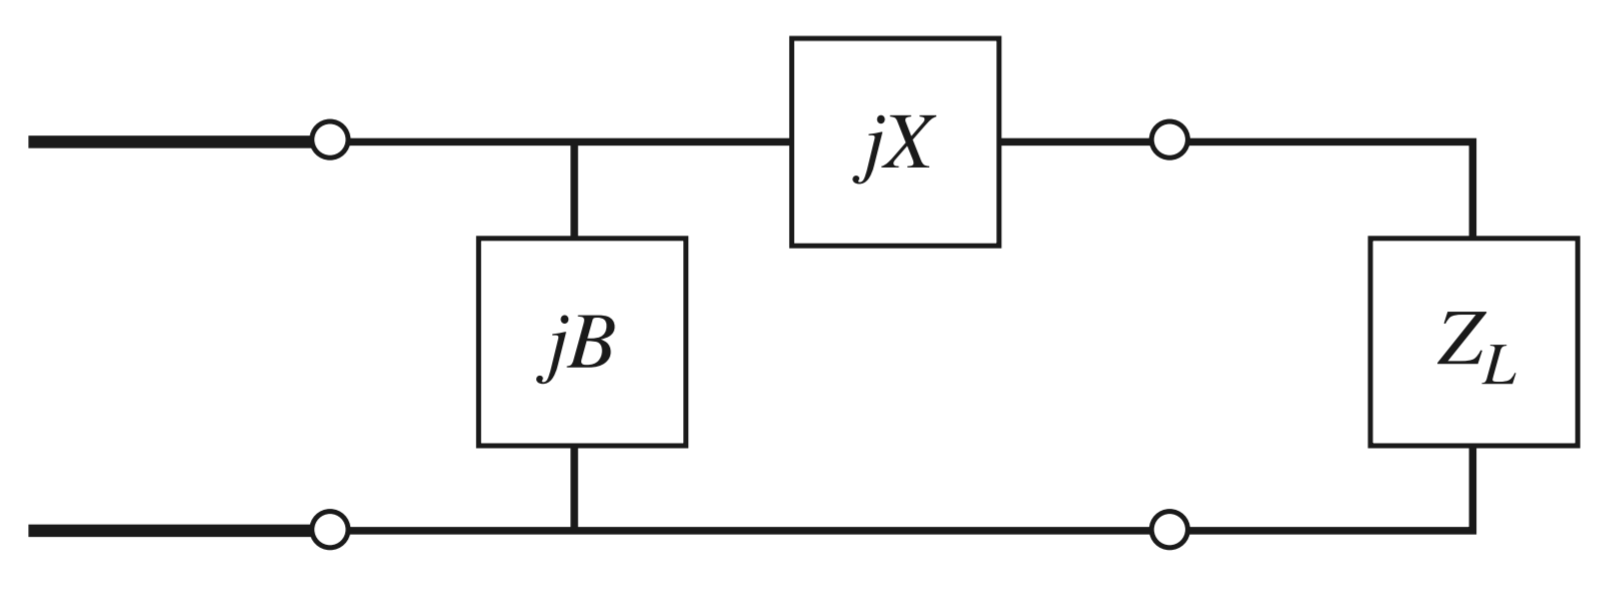
\includegraphics[height=0.3\textwidth,keepaspectratio]{figures/L-sectionmatching}
\captionof{figure}{\label{fig:L-sectionmatching}\textbf{The L-section matching circuit}. The impedance matching components are $Z_{v1}=jX$ and $Z_{v2}=jB$ where the notation convention $j$ is used to indicate an imaginary $i$. The quantum dot components are simplified to $Z_{L}$ \cite{pozar2004microwave}.}
\end{Figure}
% % 
% % 
%\subsubsection{\label{subsubsec:Heuristicvaractoroptimisation}Heuristic varactor optimisation}
We also numerically studied the response of the circuit to varying capacitances, parasitic capacitances and resistive losses. Initially $C_{v2}$ was set to $8.19$ pF and $C_{v1}$ was sweept to determined the dynamic range of 3-30 pF. The resonances range between 583-623 MHz providing a tune-ability around $f_{0}=600$ MHz of $\approx \pm 20$ MHz. Therafter, $C_{v2}$ is tuned to maximise impedance matching for $\mr{Abs}( R ) < 0.02$. For the dynamic range of $C_{v1}$ impedance matching is achieved where $C_{v2}$ ranges between 6.5-10.5 pF. For $C_{v1}=4.63$ pF and $f_{0}=600$ MHz impedance matching is optimised for $C_{v2}=8.19$ nF. These values are in agreement with the results calculated from Pozar's derivation. 
\par
Additionally, varying the resistive loss of the circuit between $R_{Loss}=10-20$ $\Omega$ has no significant effect of $f_{0}$ and the range of $C_{v2}$ enables impedance matching re-optimisation. However, the 15 nH difference between the simulated inductor value and the component available in the laboratory is significant. This is due to the nonlinear relationship between $C_{v1}$ and $f_{0}$ shown in Fig.~\ref{fig:f_0vsC_v1}. Consequently, $f_{0}$ is shift to 580 MHz which greatly limits the ability to tune $f_{0}$ using $C_{v1}$.  
\par
\begin{Figure}
\centering
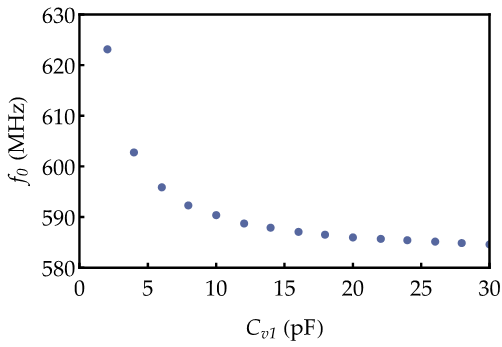
\includegraphics[height=0.5\textwidth,keepaspectratio]{figures/f_0vsC_v1}
\captionof{figure}{\textbf{Simulated resonance frequency $f_{0}$ of the circuit as a function of $C_{v_1}$}.}
\label{fig:f_0vsC_v1}
\end{Figure}
\par
\subsection{\label{subsec:Varactorgeometry}Varactor geometry}
The varactor geometry chosen to assist ease of fabricated was an interdigitated design~\cite{PhysRevB.19.3593}. Analytical simulation of the interdigitated varactor was completed using the model provided by Igreja et at. \cite{Igreja2004AnalyticalStructure}. The capacitance values calculated from this model were used to inform the dimensions of the area etched by electron-beam lithography. Thereafter, the determined capacitance values were cross-checked using a finite element software package. 
\par
The analytical results were found to significantly differ from the capacitance values derived through COMSOL simulation. Upon investigation of each method it was determined there was a mistake in the analytical model which resulted in an increase in the capacitance values by approximately a factor of two. Unfortunately this error was not detected in time to update the etching dimensions. Therefore, the varactors were fabricated with a larger capacitance than anticipated. The value of $\epsilon_{r}$ for the STO was assumed to be 23000 in the simulation.   
\par
\subsubsection{\label{subsubsection:interdigitedelectrodemodel}Interdigited electrode model}
The model developed to compute the capacitance of an interdigitated varactor can be applied to structures when the number of electrode fingers $N$ is $>$3 such that 
\begin{equation}
\label{eq:capacitanceinterdigited}
C=(N-3) \frac{C_{I}}{2}+2\frac{C_{I}C_{E}}{C_{I}+C_{E}}.
\end{equation}
\par
\noindent The capacitance of the an outer electrode relative to ground is given as $C_{E}$ while $C_{I}$ is half the capacitance of an inner electrode. This model makes the assumption of negligible electrode thickness compared to the electrode width $W$. This condition is satisfied by the fabricated varactors. Therefore, the capacitance greatly depends on the metalisation ratio
\begin{equation}
\label{eq:metalisationratio}
\eta =\frac{W}{W+G}
\end{equation}
\par
where the width of the electrode gap is $G$. Combining the contribution of capacitance from the STO sample and air determines the contribution from air is negligible. 
\par
For the geomertic dimensions given in Table \ref{tab:varactordimensions} $C_{v1}=30.3$ pF and $C_{v2}=14.8$ pF were initially outputted and used to fabricate the devices. However, following the correction to the analytical model the computed varactor capacitances are presented in Table. \ref{tab:varactordimensions} where $N=4$ for varactor $V_{2}$ and $N=8$ for varactor $V_{1}$. In Ref. \cite{Igreja2004AnalyticalStructure} the model was verified by comparison using ANSYS software to simulate a $N=4$ interdigitated capacitor. The difference in result was 1.4 \% for a $\approx$12 pF capacitor.    
\par
\vspace{1em}
\hspace*{-2em}\begin{minipage}[c]{0.45\textwidth}
%\caption{The varactor geometric dimensions and corrected capacitance values.}
\label{tab:varactordimensions}
\begin{center}
    \begin{tabular}{* {6}{l}} % <-- Changed to S here
     \toprule
      Varactor & N & $\mathcal{L}$ ($\mu$m)  & $W$ ($\mu$m) & $G$ ($\mu$m) & $C$ (pF)
      \\
      \midrule
      $V_{1}$ & 8 & 50 & 25 & 5 & 68.3 \\
      $V_{2}$ & 4 & 50 & 25 & 5 & 31.1
      \\
      \bottomrule
    \end{tabular}
  \end{center}
\end{minipage}
\par
% % 
% % 
\begin{Figure}
\centering
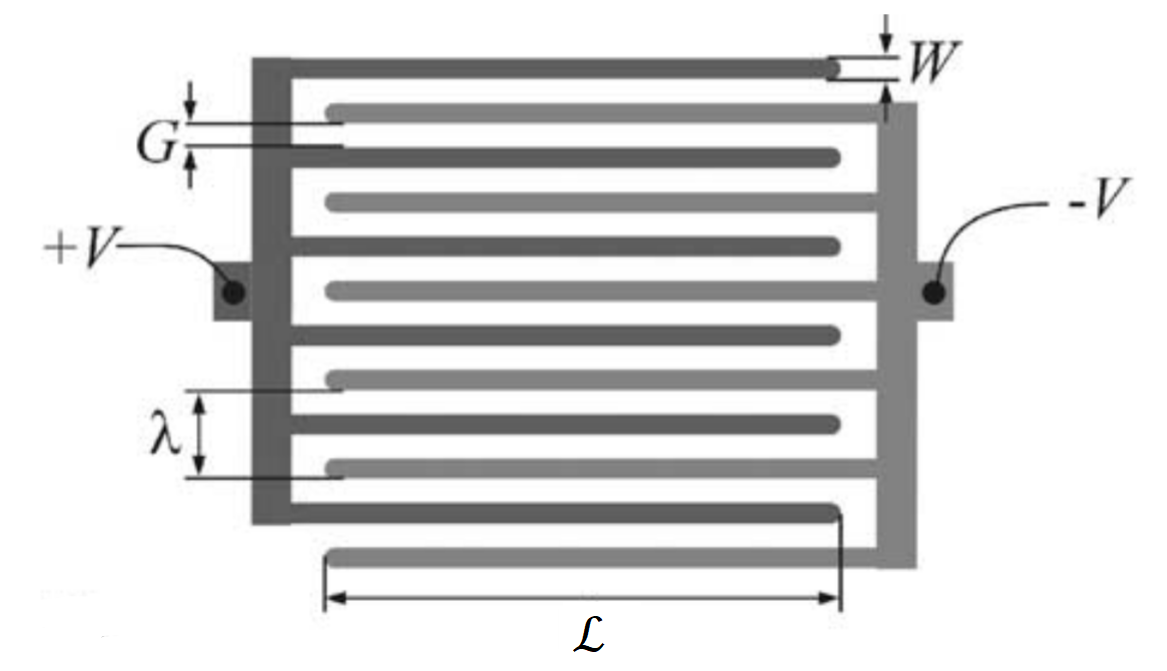
\includegraphics[height=0.5\textwidth,keepaspectratio]{figures/interdigitalvaractor}
\captionof{figure}{\label{fig:interdigitalvaractor} Varactor electrode geometry where $W$, $G$ and $\mathcal{L}$ provide the electrode width, gap size and length, respectively. \cite{Igreja2004AnalyticalStructure}.}
\end{Figure}
\par
\subsubsection{\label{subsubsec:COMSOLsimulation}COMSOL simulation}
The multi-physics software package COMSOL was utilised to provide an alternative means to calculate and verify the values of $C_{v1}$ and $C_{v2}$ for the interdigitated electrode geometries of $V_{1}$ and $V_{2}$, repsectively. The simple parallel plate capacitor tutorial \cite{COMSOLtut} was adapted to allow the electrostatic properties of the interdigitated varactors to be investigated. The geometric electrode design generated in KLayout, to enable etching of the substrate in the fabrication stage, was imported into COMSOL. The value of $\epsilon_{r}$ for the metal electrodes was approximated as 1 \cite{PhysRevB.6.4370}. 
\par
User defined meshing was applied to the device as shown in Fig.~\ref{fig:varactormeshing} where the meshing chosen determines the precision of the density of points in the simulation. The COMSOL derived values of $C_{v1}= 94$ pF and $C_{v2}= 44$ pF do not compare closely with the results shown in Table~\ref{tab:varactordimensions}. However, the simulated values of the capacitance were observed to depend strongly on the meshing applied. A factor of two increase in capacitance values were obtained when a coarse meshing was applied between the electrodes. 
\par
Additionally, for the example meshing shown in Fig. (\ref{fig:varactormeshing}) the simulated electric field is shown in Fig. (\ref{fig:electricfieldvectors}). This suggests the electric field is not modeled sufficiently with the current meshing. However, as the density of meshing increases the computational power required to complete the simulation increases. The time and memory required to run the COMSOL simulation are regarded as the limiting factors to improve the accuracy of the capacitance values outputted using this method. Measurement of the fabricated impedance matching circuit will allow properties of the varactors to be determined. This will further improve confidence in which model provides the most accurate results to advise future interdigitated capacitor fabrication.  
\par 
% % 
% % 
\begin{figure*}[b]
\centering
\begin{subfigure}[b]{0.45\textwidth}
   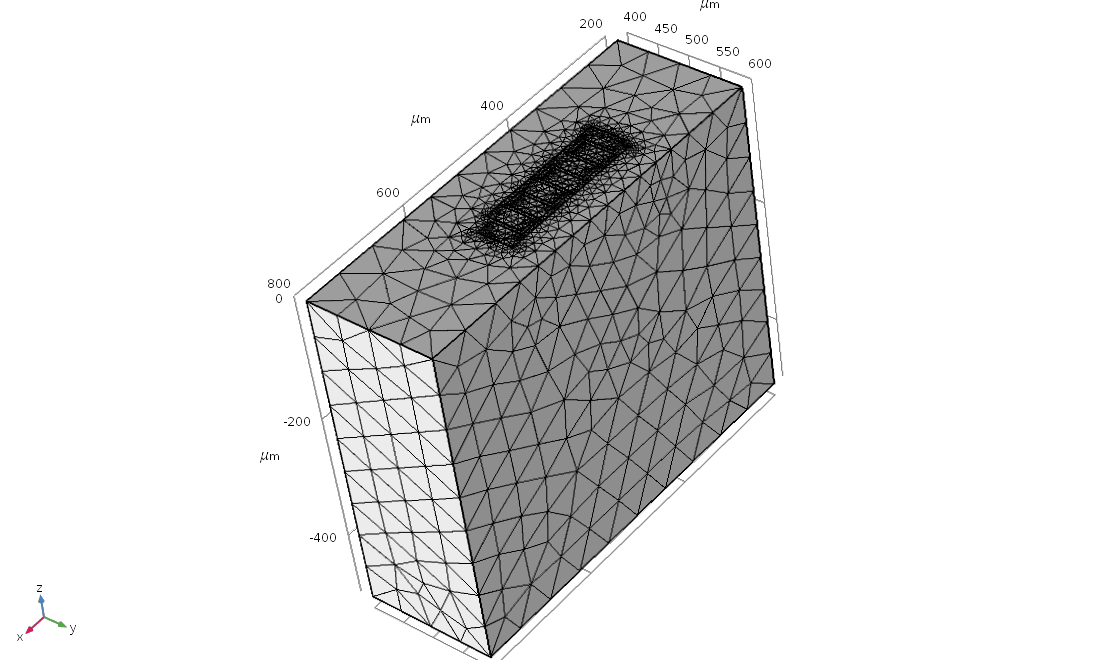
\includegraphics[width=1\linewidth]{figures/varactormeshing}
	\caption{\label{fig:varactormeshing}}
\end{subfigure}
\begin{subfigure}[b]{0.45\textwidth}
   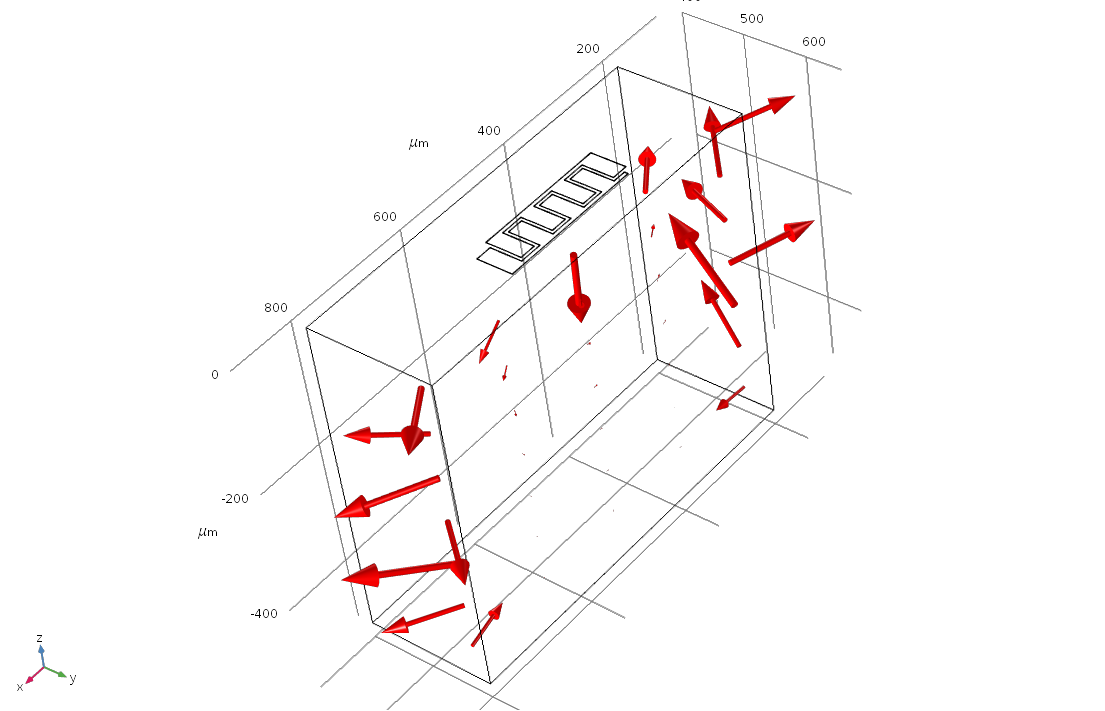
\includegraphics[width=1\linewidth]{figures/electricfieldvectors}
	\caption{\label{fig:electricfieldvectors}}
\end{subfigure}
\caption[]{(a) COMSOL meshing applied to $C_{v1}$. (b) The simulated electric field for $C_{v1}$.}
\end{figure*}
% % 
% % 
\begin{figure*}[ht]    
    \centering    
    \includegraphics[width=1\textwidth]{figures/process.png}    
    \caption{Fabrication processes step by step (3d view and cross section view):  \textcircled{1} sample preparation,  \textcircled{2} Poly methyl methacrylate (PMMA) spin coating, \textcircled{3} gold evaporation, \textcircled{4} Electron Beam Lithography (EBL) exposure, \textcircled{5} gold etching \textcircled{6} PMMA develop, \textcircled{7} Ti/Au electrode evaporation, \textcircled{8} PMMA lift-off and complete device. }
    \label{fig_process}
\end{figure*}
\section{Fabrication}
We fabricate the capacitors on a $ 0.3mm \times 0.3 mm \times 0.5\mu m$ SrTiO$_3$ (STO) substrate. 
Overview of the fabrication steps is shown in Fig. \ref{fig_process}. 
\subsection{Initial cleaning and coating}
\textbf{1. Sample cleaning}. The sample surface is proper-cleaned by its manufacturer. Thus, it suffices to rinse the substrate surface with acetone, followed by an isopropyl alcohol (IPA) treatment for the first step of the fabrication process corresponding to Fig.~\ref{fig_process}.1. The sample is placed in a so-called ultrasonic bath for 1-2 minutes, where it is soaked in the solvents. The ultrasonic vibration amplifies the effects of the cleaning chemicals. The sample was then rinsed in de-ionized water and dried with a nitrogen air flow. Acetone is used as a polar, aprotic and volatile solvent and is commonly used in laboratory cleaning processes. Metal etchants are used for samples with metal residual. Sample cleaning is completed to ensure during the transfer of sample in the clean room no influential particles remain on the surface. This cleaning process is crucial for later lithography resist coating. 
\par 
\textbf{2. Spin coating with PMMA}. Poly methyl methacrylate (PMMA) is a EBL resist where the chemical structure changes upon electron exposure. Later on, this change in chemical structure of the exposed area will be selectively removed using develop solvents. The spin coating process is completed by dropping PMMA solvent onto the sample to cover the whole surface. Thereafter, rapidly rotation of the sample forms a evenly distributed $\approx 100$ nm PMMA layer as shown in Fig.~\ref{fig_process}.2. Baking at $180$ C for 1 minute removes residual PMMA, rinse solvent, and moisture from the sample \cite{MICROCHEM}. 
\par 
\textbf{3. Gold evaporation}. The next step is to evaporate a layer of gold as shown in Fig.~\ref{fig_process}.3. This process utilises the Edwards A306 Belljar Evaporator in the London Center for Nanotechnology (LCN) to deposit a 15 nm thick layer of gold on top of the PMMA layer. In the prepared fine vacuum environment, the gold source was vaporised by resistive heating and evaporated onto the sample surface.
\par 
\subsection{Electron beam litography}
\textbf{4. EBL exposure}. Electron beam lithography (EBL) is a method of printing nano-scale structures. The varactor interdigitated geometric design was drawn in Klayout. The digital mask shown in Fig.~\ref{fig_process}.4 is used to guide selective printing through firing of electrons at specific areas of the substrate. In this process, we used the Raith 150-Two Electron Beam Lithography tool in the LCN. Due to the non-conductive PMMA substrate, we need to deposit the screening gold layer in step \textcircled{3}(Gold evaporation) to avoid inducing a charging effect. The charging effect can lead to a poor electron exposure due to Coulomb repulsion.
\par 
\textbf{5. Gold etching}. Following the completion of EBL, the screening gold layer is removed. This step corresponds to Fig.~\ref{fig_process}.5 which consists of rinsing the sample with gold acid etchant for 10s, cleaning it with IPA and drying it. The PMMA top layer substrate is now ready for the development stage. 
\par 
\textbf{6. Developement of PMMA}. The exposed PMMA can be selectively developed by Methyl isobutyl ketone (MIBK) IPA mixture(1:3) solvents for 30 seconds. The development can be stopped by placing the sample in pure IPA for 10s. After the PMMA develop process, the layout pattern is transferred onto the sample defined by trenches as shown in Fig.~\ref{fig_process}.6. 
\par 
\subsection{Titanium and gold evaporation}
This electrode evaporation is similar to the gold evaporation except this time two metal layers were evaporated: 5 nm of titanium (Ti) and followed by 60 nm gold. This is a standard gate electrode formation in which Ti can provide good adhesion to the sample surface to compensate the gold adhesion weakness. The thickness of metal deposited in trenches is the same as for the high PMMA island as shown in Fig.~\ref{fig_process}.7. The LCN Edwards A500 electron beam evaporator was used as it provides a more accurate vertical metal deposition. This reduces the metal deposition onto the vertical surfaces of the PMMA layer. The defined trenches might be wider than expected due to over-exposure and over-development, thus causing the two isolated trenches touch each other. Contact between the trenches causes a short in the final varactor. An example of this occurrence is shown in Fig.~\ref{devices} \textbf{a}.
\par 
\subsection{Lift-off and resulting devices}
The lift-off process takes off all the exposed and unexposed PMMA using an acetone bath. The sample is placed in acetone for 2 hours followed by an ultrasonic bath still within acetone solvent. The acetone does not dissolve metal but the metal on top of PMMA island will be removed with its attached PMMA. Ideally the remaining structure is the interdigitated gate electrodes as shown in Fig~\ref{fig_process}.8. The failure of the first attempt to fabricate the varactors was attributed over-development as the samples were left in the acetone solvent overnight. Conversely, uncompleted lift-off process may result in large areas of residual gold on top on sample surface as shown in Fig ~\ref{devices}b.
\par
The time taken for the several chemical steps in our experiment was either empirical or calculated by the chemical reaction rate. Specific processes should be optimized based on individual material and geometry. 
\begin{Figure}   
    \centering    
    \includegraphics[width=0.5\textwidth]{figures/optical_microscopic_images}    
    \captionof{figure}{\textbf{Optical microscope images of the device s$2$, s$31$, s$32$, and s$4$}. See table~\ref{tab_device_geometries} for the length and width of the electrodes and the gap between two electrodes (also see Fig.~\ref{fig:interdigitalvaractor}).}
    \label{fig_optical_microscopic_images}
\end{Figure}
% % 
% % 
\vspace{1em}
\begin{minipage}[c]{0.45\textwidth}
\label{tab_device_geometries}
\begin{center}
    \begin{tabular}{* {5}{l}} % <-- Changed to S here
     \toprule
      Varactor pair & $\mathcal{L}$ ($\mu$m)  & $W$ ($\mu$m) & $G$ ($\mu$m) 
      \\
      \midrule
      s$2$ & 50 & 25 & 5 
      \\
      s$31$ & 50 & 25 & 5 
      \\
      s$32$ & 50 & 50 & 10 
      \\
      s$4$ & 50 & 50 & 10 
      \\
      \bottomrule
    \end{tabular}
  \end{center}
  %\caption{The varactor geometric dimensions and corrected capacitance values.}
\end{minipage}
% % 
% % 
\section{Experimental results}
We measured two pairs of varactors, which are referred to as s$31$ and s$32$. The samples were the most well-defined in terms of visible lift-off. Room temperature four-point measurements showed no leaks through the electrodes. The gap widths are $G = 5\ \mu$m for s$31$, and $G = 10\ \mu$m for s$32$. 
For each measurement, we glued the samples to the PCB, and wire-bonded them according to the circuit shown in Fig.~\ref{fig_rf_reflectometry_setup} using aluminium wire. Note that for the measurements of s$32$, we fixed the effective $C_{\mr{p}}$ by capacitively shunting the inductor with a capacitance $C = 5$ pF $\gg C_{\mr{p}}$. By fixing $C_{\mr{p}}$, we decrease the number of parameters to be fitted from the resulting data. We cooled the samples in a dilution cryostat down to $3$ K, below which the STO dielectric constant is not expected to change, and performed RF spectroscopy as a function of $V_{\mr{frequency}}$, which we expect to tune $C_{v_1}$, and $V_{\mr{matching}}$, which we expect to tune $C_{v_2}$. 
% what was the glue?
\par
Figures~\ref{fig_spectroscopy_plots_1} and~\ref{fig_spectroscopy_plots_2} display the resulting absolute values and arguments of the reflection coefficient for s$31$ and s$32$, respectively. The operating points, i.e. the resonance frequencies, are found to be around $670...672$ MHz (see Figs.~\ref{fig_spectroscopy_plots_1} \textbf{(a)}-\textbf{(d)}) and $140...144$ MHz (see Figs.~\ref{fig_spectroscopy_plots_2} \textbf{(a)}-\textbf{(d)}), respectively. The difference in the mean is caused by the strong dependence on the parasitic or the effective parasitic capacitance. That is, $1/\sqrt{L \times 0.215 \times 10^{-12}}/(2\pi) \approx 669$ MHz, while $1/\sqrt{L \times 5 \times 10^{-12}}/(2\pi) \approx 138$ MHz. The former gives a rough starting point for estimating $C_{\mr{p}}$ in this circuit. 
\begin{Figure}
\centering 
\includegraphics[width=0.95\textwidth]{figures/vna_plot}
\captionof{figure}{\textbf{Initial spectroscopy on the vector network analyser.} Absolute value of the reflection coefficient as a function of drive frequency, showing the resonance affected by the varactors (highlighted by the blue circle), and the signal background characteristic to the setup.}
\label{fig_vna_plot}
\end{Figure}
\par
We observe three resonances between dc and $950$ MHz (see Fig.~\ref{fig_vna_plot}). By sweeping the gate voltages for tuning the varactors, we observe that two are spurious resonances that do not visibly change as a function of the voltages. In both measurements, the resonance frequency exhibits a small tuneability as a function of $V_{\mr{frequency}}$ (see Figs.~\ref{fig_spectroscopy_plots_1} \textbf{(a)}-\textbf{(b)} and~\ref{fig_spectroscopy_plots_2}\textbf{(a)}-\textbf{(b)}). The smallness in the response is likely caused by poorly chosen capacitances with respect to the inductor, which easily leads to operating at the flatter regime in the $(C_{v_1},f_0)$ plane. Current starts to leak through the capacitor electrodes above $\pm 10$ V for s$31$, and above $\pm 15$ V for s$32$. In agreement with Ref.~\cite{davidovikj2017quantum}, the first application of voltage decreases the maximal value of the dielectric constant for long timescales compared to measurement times, hence reducing the range of possible values in subsequent measurements. The slight asymmetry about $V_{\mr{frequency}} = 0$ V may be caused by an offset voltage in the case of s$31$. For s$32$, we note that the resonance is highly asymmetric around the resonance frequency, which is caused by losses in the circuit. 
\par
In the measurements of s$31$, we observe no large dependence on $V_{\mr{matching}}$. The reason for this is not well understood, but can be caused by e.g. an unexpectedly connected circuit around the smaller varactor, or damage in the varactor. We note that e.g. the wire bonds for s$31$ were not ideal in height, and could have caused a short to the sample holder and so to ground. For s$32$ both varactors responded to applied voltage. We were able to demonstrate perfect matching, which can be seen as a so-called triple point in the argument of the reflection coefficient (see Fig.~\ref{fig_spectroscopy_plots_2} \textbf{(d)}). At this point, the reflection coefficient obtains a phase shift by $2\pi$ as a function of frequency, but also as a function of applied voltage. The best matching, i.e. smallest value of $\mr{Abs}(R)$ measured was $-47.26$ dB. 
\begin{figure*}[t]
  \centering
  \textbf{(a)} \hspace{10em} \textbf{(b)}
  \\
  \includegraphics[width=0.48\textwidth]{figures/abs_R_4_6_frequency.pdf}
  \includegraphics[width=0.48\textwidth]{figures/arg_R_4_6_frequency.pdf}
  \\
  \vspace{-1em}\textbf{(c)} \hspace{10em} \textbf{(d)} 
  \\
  \includegraphics[width=0.48\textwidth]{figures/abs_R_4_6_matching.pdf}
  \includegraphics[width=0.48\textwidth]{figures/arg_R_4_6_matching.pdf} 
  \caption{\textbf{RF spectroscopy of a pair of $10\ \mu$m gap varactors.} The reflection coefficient of the sample s$31$ as a function of $V_{\mr{frequency}}$ in \textbf{(a)}-\textbf{(b)}, and $V_{\mr{matching}}$ in \textbf{(c)}-\textbf{(d)}, respectively.} 
  \label{fig_spectroscopy_plots_1}
\end{figure*}
% % 
% % 
\begin{figure*}[t]
  \centering
  \textbf{(a)} \hspace{10em} \textbf{(b)} 
  \\
  \includegraphics[width=0.48\textwidth]{figures/abs_R_9_6_frequency.pdf}
  \includegraphics[width=0.48\textwidth]{figures/arg_R_9_6_frequency.pdf} 
  \\
  \textbf{(c)} \hspace{10em} \textbf{(d)} 
  \\
  \includegraphics[width=0.48\textwidth]{figures/abs_R_9_6_matching.pdf}
  \includegraphics[width=0.48\textwidth]{figures/arg_R_9_6_matching.pdf} 
  \caption{\textbf{RF spectroscopy of a pair of $5\ \mu$m gap varactors.}  The reflection coefficient of the sample s$32$ as a function of $V_{\mr{frequency}}$ in \textbf{(a)}-\textbf{(b)}, and $V_{\mr{matching}}$ in \textbf{(c)}-\textbf{(d)}, respectively.} 
  \label{fig_spectroscopy_plots_2}
\end{figure*}
% % 
% % 
\section{Conclusions and outlook}
We measured two pairs of capacitors, intended to operate as varactors to impedance match a dispersive readout circuit used to read out the spin states of QD qubits. We demonstrated that both pairs of capacitors behaved as varactors at $3$ K. We found the perfect matching operation point for the second measured interdigitated pair of capacitors, with $N = 8$ and $N = 4$ electrodes, and a metallisation ratio of $5/6$. Tuneability in the resonance frequency was much smaller than intended, $2$ and $4$ MHz for the different measured pairs. We expect that this is partly caused by larger than intended capacitances. 
\par
We list three main sources of errors, which are to be improved in a future iteration of devices. \textbf{1.} A posteriori, the parasitic capacitance $C_{\mr{p}}$ is estimated to be close to $0.15-0.21$ pF, which was lower than the values $0.2-0.4$ pF used in numerical simulations. \textbf{2.} Modelling issues. Due to time constraints, we were able to cross-check analytically estimated capacitances with COMSOL only during and after fabrication. We found that the capacitances given by COMSOL were $1.5$ times larger than those given by analytic estimates. \textbf{3.} Due to miscommunication, we optimised values for $L = 255$ nH, which was not available for our experiment. Instead, we employed an inductor with $L = 270$ nH. 
\par
Next, the values of the capacitances at zero bias voltages should be estimated by fitting the reflection coefficient to the available data. The resulting values can be compared to the values calculated analytically and with COMSOL. If they are close to either, the effective value of the dielectric constant can be worked out. It will also help engineering more accurate maximum capacitances for future devices. Similar fits can then be performed at each value of the bias voltages to give an idea of the capacitance tuneability. Some challenges may be expected due to the small observed shifts in resonance frequency. Likewise, the readout times should be estimated for realistic values of parameters. 
\par
After amending the device as stated, the next step would be to include a Josephson parametric amplifier (JPA) in the readout circuit, tweaking the resonance of the circuit to $600$ MHz with the varactors will enable the best performance of the JPA. Use of a JPA should drastically improve the signal to noise ratio as reported in \cite{jpa}. Looking further ahead still, another use of the resonance tuning could be to tune 2 qubits to the same frequency, allowing measurement induced entanglement at a distance. Entangling measurements have been realised in superconducting qubits \cite{scmeas}, and would be an invaluable tool for quantum dot based quantum networks. 
\end{multicols}
\printbibliography
\end{document}
